
%(BEGIN_QUESTION)
% Copyright 2006, Tony R. Kuphaldt, released under the Creative Commons Attribution License (v 1.0)
% This means you may do almost anything with this work of mine, so long as you give me proper credit

An RTD measures the temperature of saturated steam at the steam drum of a boiler:

$$\includegraphics[width=15.5cm]{i04252x01.eps}$$

The RTD connects to a bridge circuit via three wires, to register temperature at a sensitive voltmeter mechanism in the control room:

$$\includegraphics[width=15.5cm]{i04252x02.eps}$$

Suppose the boiler operator decides to increase the pressure of the boiler over a period of time.  Identify the effects this pressure change will have on these voltage drops in the RTD circuit:

\begin{itemize}
\item{} $V_{R1}$ will {\it increase}, {\it decrease}, or {\it stay the same}?
\item{} $V_{R2}$ will {\it increase}, {\it decrease}, or {\it stay the same}?
\item{} $V_{R3}$ will {\it increase}, {\it decrease}, or {\it stay the same}?
\item{} $V_{RTD}$ will {\it increase}, {\it decrease}, or {\it stay the same}?
\item{} Explain the relationship between boiler pressure and boiler temperature:
\end{itemize}

\underbar{file i04252}
%(END_QUESTION)





%(BEGIN_ANSWER)

\begin{itemize}
\item{} $V_{R1}$ will {\bf stay the same}
\item{} $V_{R2}$ will {\bf stay the same}
\item{} $V_{R3}$ will {\bf decrease}
\item{} $V_{RTD}$ will {\bf increase}
\item{} Explain the relationship between boiler pressure and boiler temperature:
\end{itemize}
{\it Boiler pressure and boiler temperature are directly related: as pressure increases, temperature also increases.}

%(END_ANSWER)





%(BEGIN_NOTES)

\vskip 20pt \vbox{\hrule \hbox{\strut \vrule{} {\bf Virtual Troubleshooting} \vrule} \hrule}

This question is a good candidate for a ``Virtual Troubleshooting'' exercise.  Presenting the diagram to students, you first imagine in your own mind a particular fault in the system.  Then, you present one or more symptoms of that fault (something noticeable by an operator or other user of the system).  Students then propose various diagnostic tests to perform on this system to identify the nature and location of the fault, as though they were technicians trying to troubleshoot the problem.  Your job is to tell them what the result(s) would be for each of the proposed diagnostic tests, documenting those results where all the students can see.

During and after the exercise, it is good to ask students follow-up questions such as:

\begin{itemize}
\item{} What does the result of the last diagnostic test tell you about the fault?
\item{} Suppose the results of the last diagnostic test were different.  What then would that result tell you about the fault?
\item{} Is the last diagnostic test the best one we could do?
\item{} What would be the ideal order of tests, to diagnose the problem in as few steps as possible?
\end{itemize}


%INDEX% Measurement, temperature: RTD (bridge circuit)

%(END_NOTES)


